\documentclass[12pt]{article}

\setlength\parindent{0pt}
\newcommand{\myt}[1]{\textbf{\underline{#1}}}

\usepackage{mathtools}
\usepackage{amssymb}
\usepackage{graphicx}

\title{\vspace{-15ex}Math 239 Lecture 16\vspace{-1ex}}
\date{June 12, 2015}
\author{Graham Cooper}

\begin{document}
	\maketitle
	\section*{Graph Theory}
	Note:\\
	\begin{enumerate}
		\item A shorthand for \{u,v\} is uv.
		\item The edges are unordered, uv = vu, if order matters then it is a directed graph, draw lines with arrows
		\item We mostly consider "simple" graphs, ie no multiple edges and no loops. Loops are a nod pointing at itself, multiple edges are more than one edge between two nodes
		\item All Graphs we consider are finite
		\item Usually we don't consider empty graphs
	\end{enumerate}
	
	\subsection*{Degree}
	Definition: The degree of a vertex v is the number of edges incident with v, denoted deg(v)\\
	
	Example: \\
	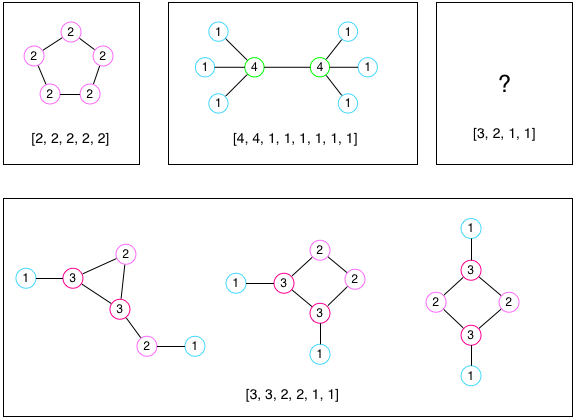
\includegraphics[scale=0.5]{degree_seq_graphs.png}
	
	Sum of the vertices of the bottom right graph
	$$\sum_{v \in V(G)} deg(v) = 12$$
	The sum will always be even, because it is the number of edges x 2\\
	
	Handshaking lemma: For any graph G, $\sum_{v \in V(G)}deg(v) = 2|E(G)|$\\
	
	Proof: Each edge uv contributes 2 to the sum, 1 for deg(u) and 1 for deg(v)\\
	
	Corollary: For each graph, the nmber of odd-degree vertices is even\\
	Proof: Let O, E be the vertices of odd and even degrees respectively. Then:\\
	$$\underset{A}{\sum_{v \in V(G)}deg(v)} = \underset{B}{\sum_{v \in O}deg(v)} + \underset{C}{\sum_{v \in E}deg(v)}$$
	
	A is even by the handshaking lemma\\
	C is even since it is a sum of even numbers.\\
	$\therefore$ B is even, Since B is a sum of odd numebrs,there must be an even numbers of them so $|O|$ is even.\\
	
	\section*{Isomorphism}
	
	Definition: Two graphs $G_1$, $G_2$ are isomorphic. If there exists a bijection $f: V(G_1) \rightarrow V(G_2)$ such that $uv \in E(G_1)$ if and only if f(u)f(v) $\leftarrow$ $E(G_2)$ (adjacency is preserved). Such  a mapping f is called an isomorphism.\\
	
	Example:\\
	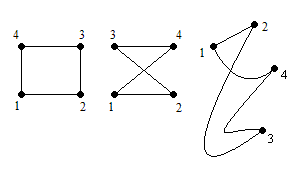
\includegraphics[scale=0.5]{isomorphic.png}
	
	
	
	
\end{document}
